\documentclass[letterpaper,10pt]{article}

\usepackage{titling}
\usepackage{listings}
\usepackage{url}
\usepackage{setspace}
\usepackage{subfig}
\usepackage{sectsty}
\usepackage{pdfpages}
\usepackage{colortbl}
\usepackage{multirow}
\usepackage{multicol}
\usepackage{relsize}
\usepackage{amsmath}
\usepackage{wasysym}
\usepackage{fancyvrb}
\usepackage{amssymb}
\usepackage{ifsym}
\usepackage{amsmath,amssymb,amsthm,graphicx,xspace}
\usepackage[titlenotnumbered,noend,noline]{algorithm2e}
\usepackage[compact]{titlesec}
\usepackage{XCharter}
\usepackage[T1]{fontenc}
\usepackage{tikz}
\usetikzlibrary{arrows,automata,shapes,trees,matrix,chains,scopes,positioning,calc}
\tikzstyle{block} = [rectangle, draw, fill=blue!20, 
    text width=2.5em, text centered, rounded corners, minimum height=2em]
\tikzstyle{bw} = [rectangle, draw, fill=blue!20, 
    text width=4em, text centered, rounded corners, minimum height=2em]

\definecolor{namerow}{cmyk}{.40,.40,.40,.40}
\definecolor{namecol}{cmyk}{.40,.40,.40,.40}

\let\LaTeXtitle\title
\renewcommand{\title}[1]{\LaTeXtitle{\textsf{#1}}}


\newcommand{\handout}[5]{
  \noindent
  \begin{center}
  \framebox{
    \vbox{
      \hbox to 5.78in { {\bf ECE356: Database Systems } \hfill #2 }
      \vspace{4mm}
      \hbox to 5.78in { {\Large \hfill #4  \hfill} }
      \vspace{2mm}
      \hbox to 5.78in { {\em #3 \hfill} }
    }
  }
  \end{center}
  \vspace*{4mm}
}

\newcommand{\lecture}[3]{\handout{#1}{#2}{#3}{Lecture #1}}
\newcommand{\tuple}[1]{\ensuremath{\left\langle #1 \right\rangle}\xspace}

\addtolength{\oddsidemargin}{-1.000in}
\addtolength{\evensidemargin}{-0.500in}
\addtolength{\textwidth}{2.0in}
\addtolength{\topmargin}{-1.000in}
\addtolength{\textheight}{1.75in}
\addtolength{\parskip}{\baselineskip}
\setlength{\parindent}{0in}
\renewcommand{\baselinestretch}{1.5}
\newcommand{\term}{Winter 2018}

\singlespace


\begin{document}

\lecture{ 26 --- Timestamp, Validation, \& Multiversion Protocols }{\term}{Jeff Zarnett}

\section*{Concurrency via Timestamps}

Beyond just doing concurrency through some sort of locking protocol, we can also use timestamps for arranging concurrency. The timestamp, as you will recall, is a unique identifier, and they are typically assigned in the order the transactions are submitted to the system~\cite{fds}. If timestamps are used appropriately, then consistent results are produced without the use of any locks or locking, meaning deadlock can never occur.

The notation for the timestamp of a transaction $T$ is $T\!S(T)$. The transactions can be ordered based on their timestamps; if a transaction $T_{i}$ arrives and then later another transaction $T_{j}$ arrives, then $T\!S(T_{i}) < T\!S(T_{j})$. If two transactions arrive at exactly the same time, then some sort of serialization procedure will be needed to make sure that they are not identical. It is commonly the case that the system clock is used to get the time stamp; just read the current value of the clock and use that.

The alternative is a logical counter: increment a simple integer counter for each transaction. After a timestamp is assigned, just increment the counter. Eventually there is a limit (even if you can have $2^{64}$ transactions, in theory, which is quite a lot, but not infinite) but at some point the transaction counter will need to roll over or reset.

Generation of the timestamps is fairly simple, it would seem, but what are they for? Timestamps are used for serializability order in the schedule; the system must ensure that the schedule executed is equivalent to a serial schedule in which transactions are ordered according to their timestamps (ascending)~\cite{dsc}. Note that this is very different from two-phase locking. In two phase locking, a schedule is serializable by being equivalent to some schedule that is permitted under the locking rules; in timestamp ordering the schedule is equivalent to the a particular serial ordering matching ascending transaction timestamps~\cite{fds}.

Every data element in the database is associated with separate timestamps for reading and writing. The notation can vary: in~\cite{fds} they are called \textbf{read\_TS} and \textbf{write\_TS}; in~\cite{dsc} they are \textbf{r-timestamp} and \textbf{w-timestamp}. To save space I might personally like $T\!S_{r}$ and $T\!S_{w}$. Each time the a data element $X$ is read or written, its appropriate timestamp is updated to the timestamp of the transaction performing the read or write.

The formal definition of the read timestamp of an item $X$: the largest timestamp amongst all the timestamps of transactions that have successfully read $X$. So $T\!S(X) = T\!S(T_{k})$ where $T_{k}$ is the youngest transaction that has read $X$ successfully~\cite{fds}.

The formal definition of the write timestamp of an item $X$: the largest timestamp amongst all the timestamps of transactions that have successfully written $X$. So $T\!S(X) = T\!S(T_{k})$ where $T_{k}$ is the youngest transaction that has written $X$ successfully~\cite{fds}.

Unfortunately, simple timestamp ordering does not avoid the risk of cascading rollback. Schedules are not guaranteed to be recoverable. This leads us to the \textit{timestamp ordering protocol} as described in~\cite{dsc}.

For a read operation $T_{i}$ is performing on $X$:
\begin{enumerate}
	\item If $T\!S(T_{i}) < T\!S_{w}(X)$ then $T_{i}$ needs to read a value of $X$ that was already overwritten -- and therefore the read operation is not permitted and $T_{i}$ is rolled back.
	\item If $T\!S(T_{i}) \geq T\!S_{w}(X)$ the read operation is executed and $T\!S_{r}$ is set to $\max ( T\!S(T_{i}),~T\!S_{r}(X))$.
\end{enumerate}

For a write operation $T_{i}$ is performing on $X$:
\begin{enumerate}

\item If $T\!S(T_{i}) < T\!S_{r}(X)$ then the value that $T_{i}$ is producing was needed previously but the system assumed it wasn't going to happen and proceeded without it; thus the write is not permitted and $T_{i}$ is rolled back.
\item If $T\!S(T_{i}) < T\!S_{w}(X)$ then $T_{i}$ is attempting to write an obsolete value; the write is not permitted and $T_{i}$ is rolled back.
\item Otherwise, the write proceeds and $T\!S_{w}(X)$ is updated to $T\!S(T_{i})$. 

\end{enumerate}

When a transaction is rolled back and restarted, the transaction is assigned a new timestamp. The timestamp ordering protocol does provide us with conflict serializability, because conflicting operations are processed in timestamp order. Because there are no locks, there cannot be deadlocks -- but can starvation still occur? The answer is yes, a very long transaction might be constantly frustrated by shorter transactions constantly swooping in and making changes that force a rollback of the long transaction. Unfortunately it might be necessary to block other transactions and let the long one finish~\cite{dsc}.

In the example below, transaction $T_{25}$ reads values $A$ and $B$ , and transaction $T_{26}$ modified both $A$ and $B$:

\begin{center}
	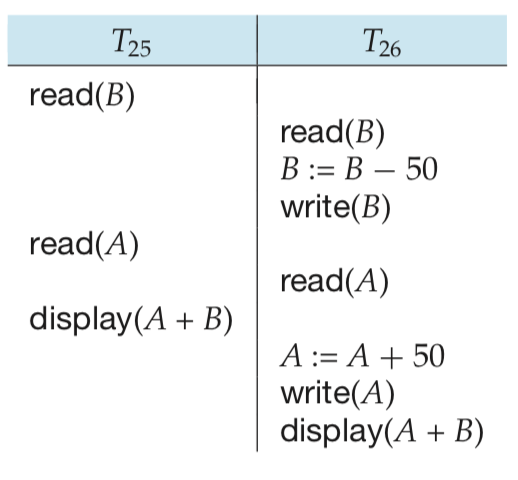
\includegraphics[width=0.3\textwidth]{images/timestamp-schedule}\\
	A schedule produced with timestamp ordering~\cite{dsc}.
\end{center}

It is worth noting that neither two phase locking nor the simple timestamp ordering protocol covers all serializable schedules; that is, there are some that are valid under one but not valid under the other~\cite{fds}. That's fine, as far as we are concerned -- we don't need to consider all possibilities; we will get enough choices.

If we would like to recoverability we can have strict timestamp ordering. In strict timestamp ordering, a transaction $T_{i}$ that issues a read or write of an item $X$ where $T\!S(T_{i}) > T\!S_{w}(X)$, then the read or write operation is delayed until the transaction that last wrote $X$ has either committed or aborted. This, in some way, requires simulating locking item $X$ until a previous write has been committed or aborted, but there cannot be a deadlock because a transaction can only wait on an older transaction (one with a  lower timestamp)~\cite{fds}.

\paragraph{Thomas's Write Rule.} A modification of the basic algorithm called Thomas's Write Rule (or the Thomas\footnote{Named after the author of the paper describing this rule, Robert H. Thomas} Write Rule) allows greater concurrency than the basic algorithm and also, hopefully, rejects fewer writes. To explain it simply, it is ``ignore outdated writes''.

More formally, the write item checks are modified to the following~\cite{fds}:
\begin{enumerate}
	\item If $T\!S_{r}(X) > T\!S(T_{i})$ then abort and roll back $T_{i}$ (write rejected).
	\item If $T\!S_{w}(X) > T\!S(T_{i})$, then do not execute the write, but continue executing (do not roll back the transaction).
	\item Otherwise, the write proceeds and $T\!S_{w}(X)$ is updated to $T\!S(T_{i})$. 
\end{enumerate}

This requires some explanation. If a transaction $T_{i}$ is going to write an old value, under the previous scheme that write would be rejected. Under Thomas's Write Rule, we will just skip doing the write (the value to be written is outdated) and we just carry on. Essentially we just pretend that the write happened but was immediately overwritten by the more up to date value. 

\section*{Validation-Based Protocols}

As you know, a transaction that is read-only does not interfere with any other read-only transaction. If a database has many more reads than writes, then a concurrency control routine might do a lot of really unnecessary work and maybe delay transactions unnecessarily. If we could instead just step in where transactions may be in conflict, that would be better, but it is necessary then to find out what transactions are the ones that have the potential for conflict...~\cite{dsc}.

The validation protocol means that transactions have three phases (although read only transactions skip the last one). The phases are described in~\cite{dsc} as:

\begin{enumerate}
	\item \textbf{Read Phase.} The transaction is executed, reading the value of items and storing them in temporary variables local to that transaction. Writes are also done on temporary local variables without any changes to stored data.
	\item \textbf{Validation Phase.} A validation test is applied (described below). If the transaction passes the test, it may proceed to step 3; if it fails, then the transaction is aborted.
	\item \textbf{Write Phase.} The temporary local variables are written written out. Obviously, read-only transactions have nothing to do in this phase and may skip it altogether.
	
\end{enumerate}

The validation test for the current transaction $T_{i}$, for each transaction $T_{k}$ where $T\!S(T_{k}) < T\!S(T_{i})$, one of the following conditions must hold:

\begin{enumerate}
	\item $T_{k}$ finishes before the start of $T_{i}$: serializability order is maintained because the current transaction starts after the previous one finished.
	\item The set of data items written by $T_{k}$ does not intersect with the set of data items read by $T_{i}$, and $T_{k}$ finishes writing before $T_{i}$ starts its validation phase. This ensures that the writes of these transactions do not overlap.
\end{enumerate} 

To make this work out as expected we need, now, three timestamps for each transaction: one for the start of the transaction, one for the start of the validation phase, and then a final timestamp for when the transaction is finished.

Validation prevents cascading rollbacks because the writes don't really take place until the validation phase has taken place. This is called \textit{optimistic concurrency control} because transactions execute optimistically, assuming that they are going to finish (and we'll sort it out if something goes wrong)~\cite{dsc}. The locking and timestamp approaches re a bit more pessimistic because they force a rollback if there is a potential for a conflict. The potential for a conflict is not a guarantee that one will occur.

That potentially leads to an interesting discussion on the subject of whether an optimistic or pessimistic type approach is better. The general recommendation is that optimistic approaches are lower overhead and better for situations where we expect there is not much contention. We get more concurrency out of optimistic schemes, which would theoretically mean better performance.

A small example to demonstrate the validation routine:

\begin{center}
	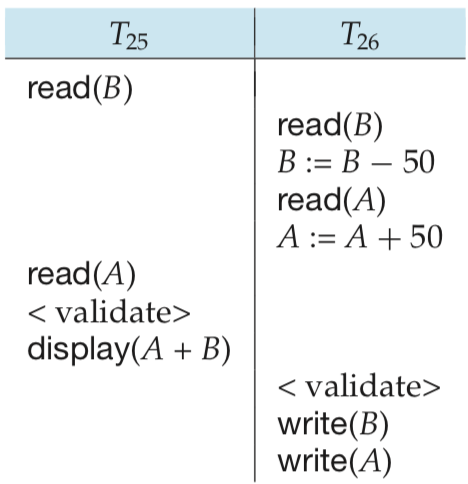
\includegraphics[width=0.3\textwidth]{images/validation}\\
	A schedule produced in a validation scheme~\cite{dsc}.
\end{center}

\section*{Multiversion Schemes}

Thus far we have said that a transaction must be either delayed or denied (aborted) to ensure serializability. In a multiversion scheme, we have multiple versions of the data at the same time; instead of rejecting a read because a write has taken place in the meantime, the read is provided an older version of the item. Choosing which one is meant to be read is the hard part of this routine, of course.

This does require more storage space to maintain multiple versions of the data. Old versions might be maintained anyway for recovery, or just record keeping purposes~\cite{fds}. Many databases are used in environments where all changes must be tracked for legal reasons, with data like the changer, change time, and what the data changed was. If that is the case then there is no additional cost to storing the data since the older versions are already present regardless. 

If that is not the case, then yes, multiple versions take extra space. The amount of space is determined by how many data items are modified, in a given period of time and how long we would like to maintain older versions. More writes means more space needed. And the longer we maintain them, the more space is needed. 

\paragraph{Timestamp Ordering.} In the multi version technique using timestamps, for a data element $X$, there are multiple versions $X_{1}, X_{2}, X_{3}, ... , X_{k}$. For each $X_{i}$ there are read and write timestamps. The read timestamp is the largest timestamp that has successfully read $X_{i}$; the write timestamp is the timestamp of the transaction that wrote the value of this version of $X$~\cite{fds}. 

Whenever a transaction is allowed to update a value, a new version of $X$ is created. As it has never been read, yet, the read timestamp should be the same as the write timestamp (until it is read of course). If a read takes place, then the read timestamp is updated if the transaction doing the read has a larger value than the current read timestamp.

Ensuring serializability requires holding to just two rules~\cite{fds}:

\begin{enumerate}
	\item If transaction $T$ tries to write item $X$, and version $i$ of $X$ has the highest write timestamp of all versions of $X$ that is also less than or equal to the timestamp of $T$, and the read timestamp of $X_{i}$ is larger than the timestamp of $T$, the abort the transaction $T$ and roll it back. Otherwise, create a new version of $X$ with read and write timestamps equal to the timestamp of $T$.
	
	\item If transaction $T$ wants to read item $X$, find the version of $X$ ($X_{i}$) that has the highest write timestamp of all versions of $X$ that is also less than or equal to the timestamp of $T$. Update the read timestamp of $X_{i}$ to the maximum of its current read timestamp and the timestamp of $T$.
\end{enumerate}

The goal is that read operations are always successful, even if they read an older version. A write, however, might not be permitted if it comes ``too late'' -- trying to write a version that another transaction would have read. The drawback is that every read requires us to update the read timestamp, which is itself a write operation (and may result in a disk access).

When do we know that we can get rid of an old version? An old version is no longer needed when its write timestamp is younger than that of the oldest transaction in the system. But one must be careful then to only delete old versions; at least the current version must be maintained. But also it means that in a period in which there are no transactions active, we may clean up any old versions. That may not occur frequently enough in a heavily used database, so it might be a periodic task to simply trash very old versions.

A major drawback of this scheme is that we resolve any conflicts on writes through rollbacks, which are expensive, rather than through waiting (which is unpleasant but tolerable)~\cite{dsc}. Then instead, an alternative:

\paragraph{Multiversion Two Phase Locking.} What if we said we want an all-of-the-above solution that combines two phase locking with the multiversion scheme? This is that solution. The advantage of multiversion schemes is that reads don't fail. The advantage of two phase locking is that locks allow transactions to wait rather than roll back, and deadlock is avoided. The plan is thus to allow each transaction to be handled in the way they like best. Thus, read-only transactions are differentiated from the update transactions.

Update transactions use two phase locking, with the restriction that they hold locks up until the end of the transaction, meaning that there his only one timestamp for the transaction, which is used to both serialize the transactions and to assign the version of the data written~\cite{dsc}. The timestamp under this scheme is an incrementing counter rather than the actual time of the transaction. 

Read-only transactions are assigned a timestamp based on the current value of the counter for update transactions, at the time when the read transaction is created. Multiple read transactions can have the same value of their timestamp. In effect, the read transaction's timestamp $k$ is declaring that its view of the data is the version at time $k$. A transaction that reads some data $X$ with its timestamp $k$ gets the version of $X$ with the largest timestamp less than or equal to $k$. 

If an update transaction wants to read an item, it acquires a shared lock on the latest version of the item; to do an update it acquires an exclusive lock and creates a new version of that item with the timestamp being the maximum value (effectively: infinity)~\cite{dsc}. The new version has this infinite timestamp so it won't be read by any read transaction, but it will be overwritten when the write transaction commits:  the commit operation sets the timestamp on all newly-modified variables to be the value of the transaction performing the update plus one. Then the timestamp counter is incremented. This does mean that only one transaction can commit at a time.

\bibliographystyle{alphaurl}
\bibliography{356}


\end{document}
